\chapter{Encounters at the Crossroads}
\index{Random Encounters}
\index{Encounters}
\index{Seasons}
\label{encounters}

\Gls{fenestra}'s institutions, structure, politics, religion, and \emph{food} all revolve around the constant problems presented by monstrous creatures wandering around the world.
These encounters encounters do not occur every hour of every day; just as deer walk through dark forests for a lifetime, so people can also visit a nearby village without certain death.
However, they will experience a \textit{reasonable danger} of death if they walk carefully, and worse if they wander carelessly.

\section{Things on the Road}

\begin{multicols}{2}

\subsection{Daily Encounters}

\begin{speechtext}
  Everyone travels together, in heavy wagons, and bows ready for action.
  But once you arrive back home, the traders finish and want to move on by morning, which doesn't leave much time to say `hello' to everyone.
  So you decide to leave with the next trading caravan, but a few days later and nobody's arrived.
  Nobody tells you to go, but when food's running low you just kinda \emph{feel} it.

  The little places by the towns don't see much danger, so if you're not too far from a big place, you might just walk to the nearest road and see if you can join a caravan heading back to town.
  Of course the bow's at the ready, and a spear if you can stand the extra weight.

  When you spot a creature, you can try to stare it down.
  If that doesn't work, give it a nasty sting and they mostly go away.
  Gotta be careful close to the cold though -- once the beasts feel the frost coming on they get \emph{fearless}.

  Once the cold settles in, the forest calms down.
  Most of the big nasty ones sleep under the snow until it melts.
\end{speechtext}

\boxPair[t]{
  \begin{encChart}{Weather}
    \Repeat{16}{
      \encLine \bigWeatherList \\
    }
  \end{encChart}
}{
  \begin{encChart}{Forest Encounter}
    \Repeat{16}{
      \encLine \bigBeastList \\
    }
  \end{encChart}
}

\begin{figure*}[b]

\bigLine

You can think of the civilization level as a line which moves down, slowly altering the encounter tables.
Past the end of the last road, the forest replaces the all traders with beasts.

\begin{multicols}{3}
\small
%%% Ex table 1
\setcounter{enc}{15}
\setcounter{diceNo}{13}
\vspace{2em}
\rowcolors{2}{}{gray!10}
\noindent
\begin{tabularx}{\linewidth}{c|L}
  \hline
  \hline
  \textbf{Roll} & \textbf{Inner Hamlets} \\
  \hline
  \Repeat{2}{
    \addtocounter{diceNo}{-1}
    \addtocounter{enc}{-1}
    \arabic{diceNo} & \bigBeastList \\
  }
  \hline
  \addtocounter{diceNo}{-1}
  \addtocounter{enc}{-1}
  \arabic{diceNo} & \ifodd\value{enc}Brigands!\else Bandits\fi \\
  \hline
  \Repeat{8}{
    \addtocounter{diceNo}{-1}
    \addtocounter{enc}{-1}
    \arabic{diceNo} & \arabic{diceNo} wagons \\
  }
  \hline
\end{tabularx}

%%% Ex table 2
\setcounter{enc}{15}
\setcounter{diceNo}{13}
\vspace{2em}
\rowcolors{2}{}{gray!10}
\noindent
\begin{tabularx}{\linewidth}{c|L}
  \hline
  \hline
  \textbf{Roll} & \textbf{The Lonely Road} \\
  \hline
  \Repeat{6}{
    \addtocounter{diceNo}{-1}
    \addtocounter{enc}{-1}
    \arabic{diceNo} & \bigBeastList \\
  }
  \hline
  \addtocounter{diceNo}{-1}
  \addtocounter{enc}{-1}
  \arabic{diceNo} & \ifodd\value{enc}Brigands!\else Bandits\fi \\
  \hline
  \Repeat{4}{
    \addtocounter{diceNo}{-1}
    \addtocounter{enc}{-1}
    \arabic{diceNo} & \arabic{diceNo} wagons \\
  }
  \hline
\end{tabularx}

%%% Ex table 3
\setcounter{enc}{15}
\setcounter{diceNo}{13}
\vspace{2em}
\rowcolors{2}{}{gray!10}
\noindent
\begin{tabularx}{\linewidth}{c|L}
  \hline
  \hline
  \textbf{Roll} & \textbf{Outer Villages} \\
  \hline
  \Repeat{9}{
    \addtocounter{diceNo}{-1}
    \addtocounter{enc}{-1}
    \arabic{diceNo} & \bigBeastList \\
  }
  \hline
  \addtocounter{diceNo}{-1}
  \addtocounter{enc}{-1}
  \arabic{diceNo} & \ifodd\value{enc}Brigands!\else Bandits\fi \\
  \hline
  \Repeat{1}{
    \addtocounter{diceNo}{-1}
    \addtocounter{enc}{-1}
    \arabic{diceNo} & \arabic{diceNo} wagons \\
  }
  \hline
\end{tabularx}

\end{multicols}

\end{figure*}

\begin{figure*}[t]
\setcounter{diceNo}{13}
\setcounter{diceNo2}{15}
\setcounter{enc}{17}

\begin{tabularx}{\linewidth}{c|c|c|LLL}
  \hline
  \hline
  \textbf{Warm} & \textbf{Mild} & \textbf{Cold} & \textbf{Forest} & \textbf{Lakeside} & \textbf{Mountains} \\
  \hline
  \encLine \bigBeastList & \encLakeside & \encMountains \\
  \encLine \bigBeastList & \encLakeside & \encMountains \\
  \encLine \bigBeastList & \encLakeside & \encMountains \\
  \encLine \bigBeastList & \encLakeside & \encMountains \\
  \encLine \bigBeastList & \encLakeside & \encMountains \\
  \encLine \bigBeastList & \encLakeside & \encMountains \\
  \encLine \bigBeastList & \encLakeside & \encMountains \\
  \encLine \bigBeastList & \encLakeside & \encMountains \\
  \encLine \bigBeastList & \encLakeside & \encMountains \\
  \encLine \bigBeastList & \encLakeside & \encMountains \\
  \encLine \bigBeastList & \encLakeside & \encMountains \\
  \encLine \bigBeastList & \encLakeside & \encMountains \\
  \encLine \bigBeastList & \encLakeside & \encMountains \\
  \encLine \bigBeastList & \encLakeside & \encMountains \\
  \encLine \bigBeastList & \encLakeside & \encMountains \\
  \encLine \bigBeastList & \encLakeside & \encMountains \\
  \hline
\end{tabularx}
\end{figure*}

\noindent
Encounters adjust, depending on the season, time of day, and how far the troupe have travelled from civilization.

\begin{itemize}
  \item
  Roll $3D6$ to check for encounters and the weather.
  \begin{description}
    \item[Die 1]
    shows how many \glspl{interval} until the next encounter.
    \item[Die 1 + die 2]
    tell you the encounter.
    \item[Die 3]
    may tell you the number appearing.
    \item[Die 2 + die 3]
    tell you the weather.
  \end{description}
  \item
  Close to a town, the civilization level is high (level 8 to 12), and it slowly decreases as one walks (7,~6,~5,~\ldots) to the outer roads (4,~3, 2,~\ldots).

  Compare your encounter roll to the civilization level:
  \begin{description}
    \item[Rolling above]
    means the beast listed below has taken an interest in the troupe.
    \item[Rolling below]
    means the players have spotted a caravan of travellers and traders.
    The encounter roll tells you how many wagons are together.
    \item[On a tie]
    outlaws attack.
    \begin{itemize}
      \item
      Odd numbers mean brigands,
      \item
      even numbers mean bandits.
      (see~\autopageref{brigands})
      \item
      Double the number rolled shows how many are present.
    \end{itemize}
  \end{description}
  \item
  At night, roll, with -1 to the encounter roll and weather rolls.
  The civilization level drops by 5.
  \item
  Once you roll an encounter, mark it off -- do not repeat it for the rest of the session.
\end{itemize}

\end{multicols}

\pagebreak

\begin{multicols}{2}

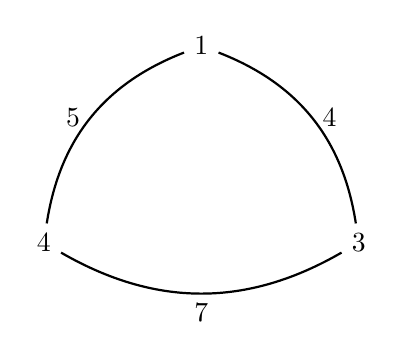
\begin{tikzpicture}[thick]

\node (A) at (0,0){\dicef{4}};

\node (B) at (4,0){\dicef{3}};

\node (C) at (2,2.5){\dicef{1}};

\draw (A) to[bend left] node[left]{5}(C) ;

\draw (C) to[bend left] node[right]{4}(B);

\draw (B) to[bend left]node[below]{7} (A);

\end{tikzpicture}

\begin{exampletext}
  \noindent
  For example, the troupe decide to head out, so you make a roll.

  \rowcolors{2}{}{}
  \begin{center}
    \begin{tabular}{cl}
    \Large\underline{\epsdice{6} \epsdice[black]{3}} & \Large\epsdice{4} \\
    9 & 4 \\
    \end{tabular}
  \end{center}

  The first two total 9,
  so the result is
  \setcounter{enc}{9}
  `\bigBeastList'.
  Use the final die for the number appearing.
  If the roll calls for a `D6', just cut the D6 in half.%

  You can see the weather in the last two dice:

  \begin{center}
    \begin{tabular}{rc}
    \Large\epsdice{6} & \underline{\Large\epsdice[black]{3} \epsdice{4}} \\
    & 7 \\
    \end{tabular}
  \end{center}

  That totals 7, meaning `\bigWeatherList'.
  The next encounter will occur 6 \glspl{interval} later.
  Since this encounter came during the day, the next will come tomorrow, at night.

  So with just 3 dice rolled, you instantly have `\bigBeastList~in the \bigWeatherList'.

\end{exampletext}


\subsection{Traders \& Nomads}

While moving, everyone meets other travellers head-on, moving in the opposite direction from them.
They briefly swap news of the road behind, occasionally make a trade, then move on.

\encTraders

Roll $3D6$ whenever the troupe encounter travellers -- every number rolled indicates something interesting to buy.

\end{multicols}


\section{Morale}
\label{morale}
\index{Morale}
\begin{multicols}{2}

\noindent
An antagonist's morale decides when a fight starts, and when it ends.

Predators don't like fair fights -- they want to pounce, subdue, and \emph{feed}.
Most predators will back off once hurt, and much of the time, they won't approach in the first place.


\begin{itemize}
  \item
  If a predator's actions seem unclear, have them roll \roll{Charisma}{Combat} (or any other martial Skill) against \gls{tn} 7.
  \item
  Beasts, who have no Charisma Attribute, must simply roll Brawl.
  \item
  The morale roll has some adjustments (see the chart).
  Most modifications grant +2 to the check when the \glspl{pc} seem weak, and -2 when they seem strong.
  \item
  A failed roll for a mindless animal might mean a chitincrawler waits and watches the party, but does not approach.

  \item
  On a tie, the enemy threatens the \glspl{pc} but takes their lead -- if the \glspl{pc} run, they attack, if the \glspl{pc} stay, they back off.
  \item
  Success means `I think I can take them', but the story does not end there.
  Once you roll the dice, keep them there.
  The bandits who felt fearless because they outnumbered the \glspl{pc} may reconsider once a few die, and they no longer outnumber the \glspl{pc}.
  \item
  Enemies only roll a single check for the group, but everyone keeps their own score.
  \item
  The \gls{gm} should keep the \glspl{npc} roll hidden.
\end{itemize}

\begin{exampletext}
  The Witch coven approach, shouting their demands arrogantly.
  The \gls{gm} has rolled only `6' for their Morale check, but most of the witches present have at least one magical sphere at +2 (a martial Skill), so they have a total of `8', and think they can take the troupe on in a fight.

  Unfortunately, a few of the apprentices' highest sphere is only at level 1, meaning they rolled a `7' -- a tie.
  And if those apprentices receive a single point of Damage, the wound will reduce them to a score of `5', and they will run, which will mean the troupe outnumber the witches, and the rest will flee on the next round.
\end{exampletext}

You can use a single roll for an entire combat -- the \gls{gm} simply keeps that roll hidden.
If the enemy rolls a `12', all of them will probably fight until they die.
If they roll a `7', they may start to flee once wounded, and then more will flee once only half remain (but they continue to recheck only at the start of a round).

Most combats will end with one side or the other running away -- few troops want to fight to the last man when they could potentially be safe at home by the end of the day.

When people fail a morale check, they often don't show any fear -- instead they become friendly.
Nobody wants to get on the bad side of someone who looks like they mean business and a bloody nose.
Of course, those people can reassess the situation.
If they \glspl{pc} take no care about their travelling companions, they may find that those `penniless traders', meant them harm all along, and just wanted to wait until the right moment to slit their throats.

The players do not take Morale checks -- they decide when it's time to run away by the look of the situation.
Usually a good time is when all the \gls{fp} have run out.
\footnote{The \glsentrytext{gm} may also wish to cut all Morale checks for any \glspl{npc} with remaining \glsentrytext{fp}.}

\moralechart

\end{multicols}

\section{Happenings \& Situations}

\begin{multicols}{2}

\subsubsection{Village Events}
\index{Villages!Events}

Roll $2D6$ for a random village event.

\encVillageEvent

\end{multicols}

\section{Missions}
\index{Adventure Generator}
\index{Missions Generator}

\begin{multicols}{2}

\noindent
\Glspl{guard} recruits can expect harsh duties.
The character with the highest rank will be asked to lead the party (ties are broken by Charisma + Deceit), and give a bonus to the first die-roll.

\begin{itemize}
  \item
  Roll $1D6$ for Fodder
  \item
  Roll $1D6+1$ for Archers
  \item
  Roll $1D6+2$ for Cutters
  \item
  Roll $1D6+3$ for Rangers
\end{itemize}

Then add a complication with the same bonus as before (\autopageref{missionComplications}).

\subsubsection{Missions}
\index{Missions}

\ngMissions

\subsubsection{Complications}
\label{missionComplications}

Add a bonus for rank, as before.

\missionComplications

\end{multicols}
